
\documentclass[]{article}
\usepackage{tikz}
\usetikzlibrary{positioning}
\usetikzlibrary{shapes.geometric, arrows}

\tikzstyle{startstop} = [
    rectangle,
    rounded corners,
    minimum width=3cm,
    minimum height=1cm,
    text centered,
    draw
]

\tikzstyle{process} = [
    rectangle,
    minimum width=3cm,
    minimum height=1cm,
    text centered,
    draw
]

\tikzstyle{decision} = [
    diamond,
    minimum width=3cm,
    minimum height=1cm,
    text centered,
    draw
]
\begin{document}

\begin{tikzpicture}
    % drawing commands
    % \draw (0,0) -- (3,0);
    % \draw (0,0) -- (2,3);
    % \draw (0,0) -- (2,0) -- (2,2) -- (0,2) -- cycle;
    % \draw (0,0) rectangle (3,2);
    % \draw[fill=blue!20] (0,0) rectangle (3,2);
    % \fill[blue!20] (0,0) rectangle (3,2); % no border
    % \filldraw[fill=yellow] (0,0) rectangle (3,2);
    % \draw (2,2) circle (1);
    % \draw (2,2) ellipse (2 and 1);
    \node at (2,2) {Hello};
    \node at (2,4) {A};
    \node[draw] at (4,2) {B};
    \node[draw] (A) at (0,0) {A};
    \node[draw] (B) at (4,0) {B};
    \draw (A) -- (B);
\end{tikzpicture}

\vspace{\baselineskip}
\smallskip
\medskip
\bigskip
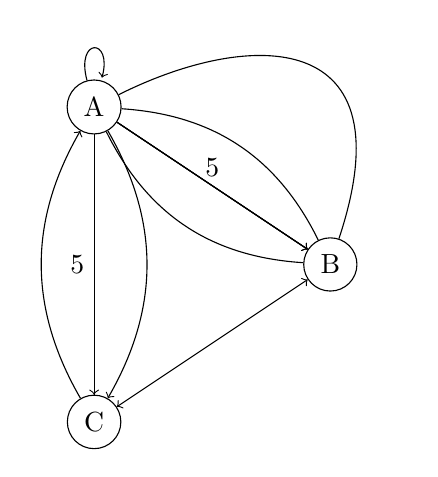
\begin{tikzpicture}

\node[circle, draw] (A) at (0,2) {A};
\node[circle, draw] (B) at (3,0) {B};
\node[circle, draw] (C) at (0,-2) {C};

\draw (A) -- (B);
\draw [<->](B) -- (C);
\draw (C) -- (A);
\draw[->] (A) -- (B);
\draw[->] (A) -- node[above] {5} (B);
\draw[->] (A) -- node[midway, left] {5} (C);
\draw (A) .. controls (2,3) and (4,3) .. (B);
\draw[bend left] (A) to (B); %uper
\draw[bend right] (A) to (B); %lower
\draw[->, bend left] (A) to (C);
\draw[->, bend left] (C) to (A);
\draw[->] (A) edge[loop above] ();
\end{tikzpicture}

\bigskip
\section*{relative positioning}
\begin{tikzpicture}
    \node (A) at (0,0) {A};
    \node (C) at (3,5) {C};
    % \node (B) at (3,0) {B};
    \node[draw, circle] (A) {A};
    \node[circle, draw] (C) at (3,5) {C};
    \node[right=2cm of A] (B) {B};
    % \draw[thick] A -- B;
    \draw[very thick, dashed] (A) -- (C);
\end{tikzpicture}
\bigskip
\section*{color}
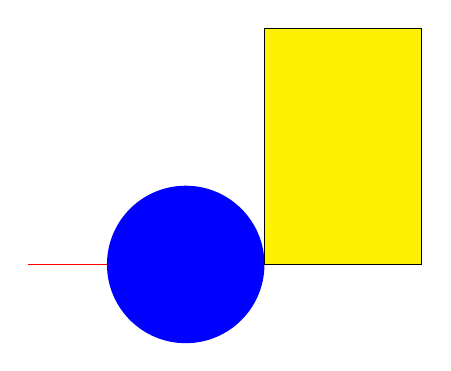
\begin{tikzpicture}
    \draw[red] (0,0) -- (3,0);
    \fill[blue] (2,0) circle (1);
    \filldraw[fill=yellow, draw=black] (3,0) rectangle (5,3);
\end{tikzpicture}
\section*{text replace, polar}
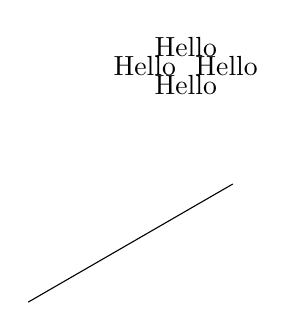
\begin{tikzpicture}
    \node[above] at (2,3) {Hello};
    \node[below] at (2,3) {Hello};
    \node[left] at (2,3) {Hello};
    \node[right] at (2,3) {Hello};
    \draw (0,0) -- (30:3);
\end{tikzpicture}

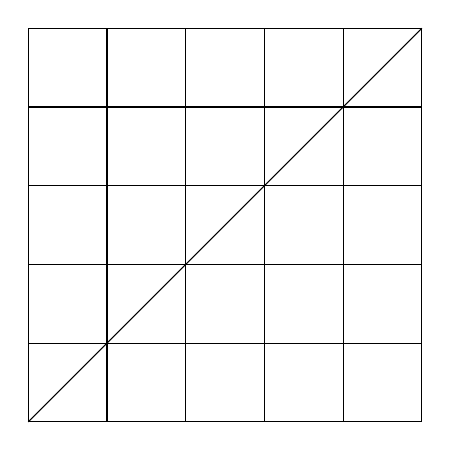
\begin{tikzpicture}
    % \draw[step=1cm, gray] (0,0) grid (5,5);
    \draw[step=1cm] (0,0) grid (5,5);
\draw (0,0) -- (5,5);
    
\end{tikzpicture}

\begin{tikzpicture}
    \draw[->] (-1,0) -- (5,0) node[right] {$x$};
\draw[->] (0,-1) -- (0,5) node[above] {$y$};
\node at (2,2) {$x^2+y^2=r^2$};
\end{tikzpicture}

\begin{tikzpicture}
    \node[circle, draw] (A) at (0,3) {A};
\node[circle, draw] (B) at (-2,1) {B};
\node[circle, draw] (C) at (2,1) {C};
\node[circle, draw] (D) at (-3,-1) {D};
\node[circle, draw] (E) at (-1,-1) {E};

\draw (A) -- (B);
\draw (A) -- (C);
\draw (B) -- (D);
\draw (B) -- (E);
\end{tikzpicture}

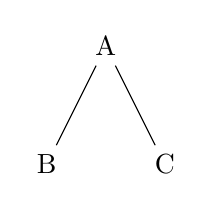
\begin{tikzpicture}
\node {A}
    child {node {B}}
    child {node {C}};
\end{tikzpicture}

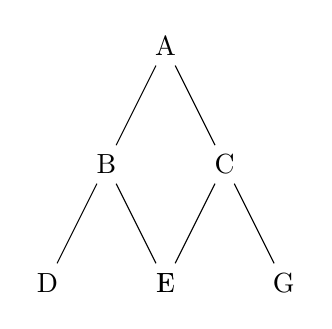
\begin{tikzpicture}
\node {A}
    child {
        node {B}
        child {node {D}}
        child {node {E}}
    }
    child {
        node {C}
        child {node {F}} % issue, F is not shown
        child {node {G}}
    };
\end{tikzpicture}

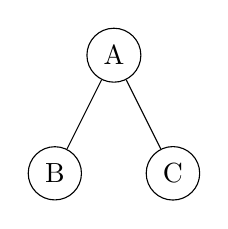
\begin{tikzpicture}
\node[circle, draw] {A}
    child {node[circle, draw] {B}}
    child {node[circle, draw] {C}};
\end{tikzpicture}

\section*{flowchart}
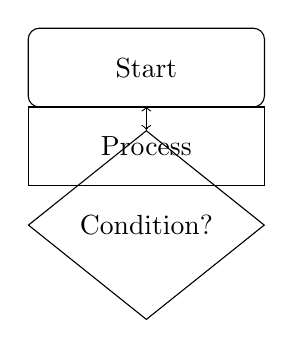
\begin{tikzpicture}
    \node[startstop] (start) {Start};
\node[process, below of=start] (process) {Process};
\node[decision, below of=process] (decision) {Condition?};

\draw[->] (start) -- (process);
\draw[->] (process) -- (decision);
\end{tikzpicture}

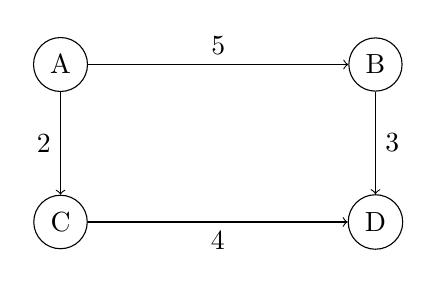
\begin{tikzpicture}

\node[circle, draw] (A) at (0,2) {A};
\node[circle, draw] (B) at (4,2) {B};
\node[circle, draw] (C) at (0,0) {C};
\node[circle, draw] (D) at (4,0) {D};

\draw[->] (A) -- node[above] {5} (B);
\draw[->] (A) -- node[left] {2} (C);
\draw[->] (B) -- node[right] {3} (D);
\draw[->] (C) -- node[below] {4} (D);

\end{tikzpicture}



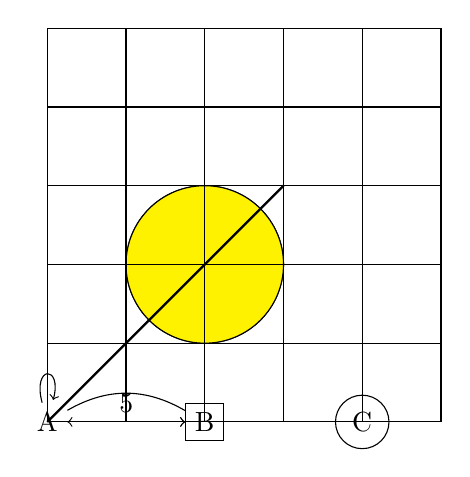
\begin{tikzpicture}

% Point/node
\node (A) at (0,0) {A};

% Box node
\node[draw] (B) at (2,0) {B};

% Circle node
\node[circle, draw] (C) at (4,0) {C};

% Line
\draw (A) -- (B);

% Arrow
\draw[->] (A) -- (B);

% Bidirectional
\draw[<->] (A) -- (B);

% Label
\draw (A) -- node[above] {5} (B);

% Rectangle
\draw (0,0) rectangle (3,2);

% Circle
\draw (2,2) circle (1);

% Filled shape
\fill[blue] (2,2) circle (1);

% Filled + outline
\filldraw[fill=yellow] (2,2) circle (1);

% Dashed
\draw[dashed] (0,0) -- (3,3);

% Thick
\draw[thick] (0,0) -- (3,3);

% Grid
\draw[step=1] (0,0) grid (5,5);

% Curve
\draw (A) to[bend left] (B);

% Loop
\draw[->] (A) edge[loop above] ();

\end{tikzpicture}

\end{document}
